\documentclass[a4paper]{article}

\usepackage{hyperref, amsmath, graphicx, float, blindtext} % for dummy text
\graphicspath{ {./images/} }
\title{Attention is all you need}
\author{Shubham Gupta}

\begin{document}
\maketitle
\section{Introduction}
\begin{itemize}
    \item This paper review is following the blog from Jay Alammar's blog on the \textbf{Illustrated Transformer}. The blog can be found \href{https://jalammar.github.io/illustrated-transformer/}{here}.  
\end{itemize}
\section{Paper Introduction}
\begin{itemize}
    \item New architecture based solely on attention mechanisms called \textbf{Transformer}. Gets rids of recurrent and convolution networks completely.  
    \item Generally, RNN used to seq-to-seq tasks such as translation, language modelling, etc.
    \item Transformer allows for significant parallelization and relies only on attention.
\end{itemize}
\section{Background}
\begin{itemize}
    \item \textit{Self attention} Attention to different positions of a sequence in order to compute a representation of the sequence.
\end{itemize}
\section{Model Architecture}
\begin{itemize}
    \item Transformer uses the following:
    \begin{itemize}
        \item Encoder decode mechanism
        \item Stacked self attention
        \item Point wise fully connected layer for encoder and decoder
    \end{itemize}
    \begin{figure}[H]
        \centering
        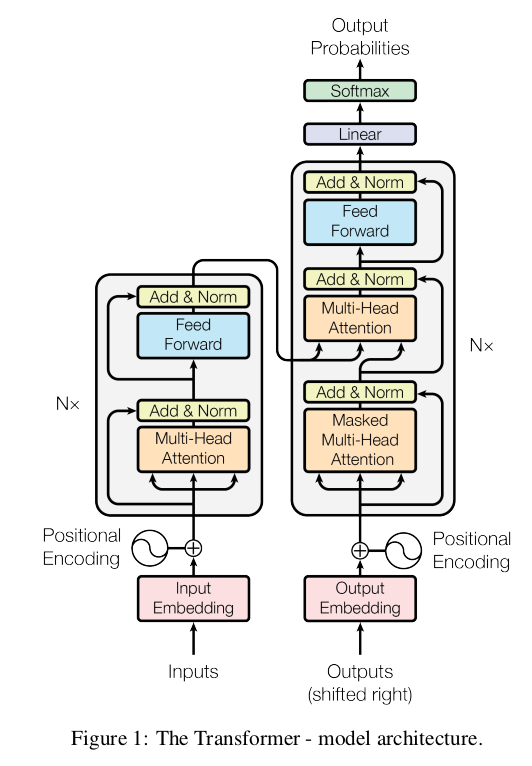
\includegraphics[width=0.8\textwidth]{transformer}
        \caption{transformer}
        \label{fig:transformer}
    \end{figure}
\end{itemize}
\subsection{Encoder and decoder stacks}
\begin{itemize}
    \item \textbf{Encoder}: 6 identical layers. 2 sub layers per layer
    \item \textit{First}: multi-head self attention mechanism
    \item \textit{Second}: Fully connected feed forward network
    \item Apply residual connection for each of the two laters
    \item Apply layer normalization
    \item \textbf{Decoder}: 6 identical layers. 2 sub layers as above + 1 more which performs multi-head attention over output of encoder stack 
    \item Resodual locks around all 3 sub layers
    \item Layer normalization
    \item Modify self-attention sub layer to prevent positions from attending to subsequent positions. Ensures that \textit{i} output depends only on words before \textit{i}.
\end{itemize}
\subsection{Attention}
\begin{itemize}
    \item 3 vectors: Query(Q), Key(K) and Value(V)
    \item Output = Weighted sum of values. Weights assigned as a function of query with key.
    \item Scaled dot-product attention and multi-head attention
\end{itemize}
\end{document}
